
\documentclass[../main.tex]{subfiles}
\begin{document}

In this chapter, we describe the Random Forest learning algorithm. We first motivate and describe decision trees, which are the basic components of a Random Forest. We then proceed to describe a particular property of decision trees: they are likely to exhibit high variance. While this is undesirable for a learning algorithm, we will see that combining several randomized decision trees into a Random Forest ensemble turns exactly that property into a crucial advantage (see section \ref{sec:unchanged-bias}).
% TODO make sure we get back to this later -- I think the idea was to say that if there's high variance, we also have high room to improve due to diversity?

In its essence, a Random Forest is a collection of randomized decision trees. A decision tree is a data-driven recursive partitioning scheme, combined with a means to produce a prediction based on the training points in a partition cell. The Random Forest prediction then is an aggregate of the predictions of all individual trees.
% TODO also don't uppercase RFs?

\section{Decision Trees}
\label{sec:decision-trees}

As described in section \ref{sec:supervised-learning}, we are interested in learning algorithms that, given some training data, produce a model that is able to predict a reasonable outcome when queried with a previously unseen example. 

% \marginnote{TODO decision tree construction pseudocode}

One intuitive approach is to consider the examples in the training data that are "close" to the query point. Then, one might claim that the outcome for the query point must surely be similar to the outcomes of the close points -- which we already know. Indeed, finding a proper notion of "closeness" is at the heart of many machine learning algorithms such as $k$-Nearest-Neigbours, $k$-Means, etc.
% TODO some examples other than k--

% TODO decision tree always lowercase
Constructing a decision tree means recursively partitioning the input space $\mathcal{X}$, guided by the training data $D$. Then, given a query $X$, we check the partition cell that $X$ belongs to and all the training examples that are in it. These are the examples we consider "close" to $X$. The tree's prediction will be an aggregation of the outcomes of all training points in that cell. 

Because we are recursively partitioning the input space, we have at hand a tree structure of decision rules. The cells of the resulting partition are the leaves of the tree. The non-leaf nodes are also referred to as \textit{decision nodes}, but there is no inherent difference between leaf and non-leaf nodes. We will use either of the terms \textit{leaf} and \textit{cell}, depending which aspect we want to emphasize.


% \marginfigfromsource{fig:decision-tree-structure}{symlinks/illustrations/decision-trees/tree-structure}

\begin{marginfigure}
    \label{fig:decision-tree-partition}
    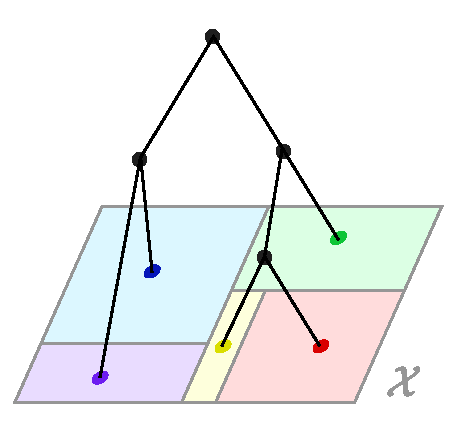
\includegraphics[width=\textwidth]{figma-illustrations/decision-tree}
    \caption{
        Rendering of a decision tree structure. Each inner node corresponds to a partitioning of the parent edge. In standard decision trees, this is a binary partition. In other words, the examples are \textit{split} at a certain value threshold in a certain feature dimension.    }
\end{marginfigure}

\marginfigfromsource{fig:decision-tree-boundaries}{symlinks/illustrations/decision-trees/decision-tree-boundaries}
    

In summary, there are the following main components to the implementation of a decision tree:
% TODO lowercase "decision tree" always
\begin{itemize}
    \item The \textit{splitting criterion} to apply recursively to subsets of the training data.
    \item The \textit{stopping criterion} that determines whether a node should be split further. This will determine the depth of the decision tree.
    \item The \textit{leaf aggregation function} that produces a prediction for a specific cell. When using the constructed tree for prediction, this will be the leaf node that the query point is assigned in.
\end{itemize}


\subsection{Centroids as leaf combiners} 

% TODO don't talk about "points"

We will consider the leaf aggregation function first. Consider a parent node $P$ that, due to some split, was partitioned into the disjoint union $L~\dot{\cup}~R$.
Let $y_{P}, y_{L}$ and $y_{R}$ be the output values of the parent and the two new leaf nodes, produced by the leaf aggregation function. Since the leaf output is constant over a single cell, the gain in loss due to a split is the difference between the loss of the parent node and the sum of losses of the two individual child nodes.
For brevity, we write $\ell_{P}(y) \defeq \sum_{i \in P} \ell(y, y_{i})$.
\begin{align*}
\text{\textit{Loss Gain}: } \hspace{1em} &
\sum_{i \in P} \ell(y_{P}, y_{i}) - \left(  \sum_{i \in L} \ell(y_{L}, y_{i}) + \sum_{i \in R} \ell(y_{R}, y_{i}) \right) \\[1.5em]
&= \ell_P(y_P) - \left(\ell_L(y_L) + \ell_R(y_R) \right)
\end{align*}
In order for a split to yield positive loss gain, the leaf aggregation function needs to be such that the loss does not increase as constraints are removed, i.e. the set of considered examples is reduced. Recall that $\bar{z}$ is a centroid with respect to a loss function $\ell$ and a set of outcomes $P$ if and only if $\bar{z} = \arg\min_{z} \sum_{i \in P} \ell(z, y_{i}) = \arg\min_z \ell_P(z)$ (\ref{prelims:centroids}).
\begin{lemma}
\label{lemma:loss-gain-nonnegative}
For a loss function $\ell$, if the leaf aggregator of a node $P$ is $y_{P} \defeq \arg\min_{z} \sum_{i \in P} \ell(z, y_{i})$, i.e. the centroid with respect to $\ell$, the loss gain is nonnegative.
% TODO double-check ~positive~ -> nonnegative.
\end{lemma}
\begin{proof}
Let $\ell_{P}(y) \defeq \sum_{i \in P} \ell(y, y_{i})$. Since $P = L \dot{\cup}R$, we need to show that $\ell_{P}(y_{P}) = \ell_{L}(y_{P}) + \ell_{R}(y_{P}) \geq \ell_{L}(y_{L}) + \ell_{R}(y_{R})$. Assume $\ell_{L}(y_{P}) < \ell_{L}(y_{L})$. This contradicts the definition of $y_{L}$ as the minimizer, and as such $\ell_{L}(y_{P}) \geq \ell_{L}(y_{L})$. Likewise, we can conclude that $\ell_{R}(y_{P}) \geq \ell_{R}(y_{R})$. Combining the two inequalities yields the statement.
\end{proof}

This rigorously motivates the specific choice of leaf aggregation function. The majority vote is a centroid with respect to the \zeroone-loss for classification, while the arithmetic mean is the centroid with respect to the squared error loss for regression.


% define stopping criteria
% defin leaf aggregations

\subsection{Splitting criteria greedily minimise loss functions}
\label{sec:splitting-criteria-greedily-minimise-loss-functions}

In the best possible case, all training examples in a given cell correspond to the same (classification) or very similar (regression) outcomes. If a query point then falls within that cell, i.e. it has similar features, one can say with high confidence that the query point should have the same (similar) outcome. In the spirit of greedy optimisation, we aim to split cells such that the resulting child cells are more \textit{pure} with respect to their outcomes. 

\marginnote{
    Note that the notion of local purity is linked to the training error: If a leaf cell is perfectly pure, all training examples in that cell correspond to the same outcome. Hence, the leaf aggregation function, which us usually implemented as some kind of mean, will produce exactly that outcome for any query point that belongs to this cell, in particular any training points. Consequently, for a suitable definition of "error", perfectly pure cells have zero training error.
}

% TODO diagram with tables, how a split makes the outcomes more pure


Consider a split, parameterised by $\Theta$, that partitions a parent node $P$ into the disjoint union $L_{\Theta} ~\dot{\cup}~R_{\Theta}$. Let $n, n_{L}, n_{R}$ be the cardinalities of the parent and the two child nodes. Let $H$ be an impurity measure. We will select the split that yields the lowest impurity.
$$
\arg \min_{\Theta} ~ \frac{n_{L}}{n} H(L_{\Theta}) + \frac{n_{R}}{n} H(R_{\Theta})
$$
The gain in purity is then the difference between impurities before and after the split.
\begin{align}
\text{\textit{Purity Gain}: } \hspace{1em}
H(P) - \left(  \frac{n_{L}}{n} H(L_{\Theta}) + \frac{n_{R}}{n}H(R_{\Theta}) \right)
\label{eq:purity-gain}
\end{align}
Note that this is different from the gain in \textit{loss} achieved due to a split. 


We now proceed to define two commonly used splitting criteria. These are the Gini impurity for classification and Variance Reduction (also known as \textsc{Cart}) for regression \cite{tibshirani_ElementsStatisticalLearning_2017}.
For a splitting function criterion to produce useful decision trees, a reasonable impurity measure should also imply a positive loss gain. Often, this is intuitively clear but particularly for the case of Gini impurity, a comprehensive explanation appears to be hard to find in the literature. We clarify this in the following.

\subsubsection{Variance Reduction}
\marginnote{In binary classification, i.e. if outcomes are in $\{0,1\}$, the squared error reduces to the \zeroone-loss. As such, the mean \zeroone-loss, i.e. the error rate, trivially also is a measure of variance.
% OK this is really quite trivial, not sure whether we should keep
}
\marginnote{
    % TODO attribute sklearn 1.10.7.1 (box) https://scikit-learn.org/stable/modules/tree.html#classification-criteria
Another impurity measure is the entropy, defined as
$$
H_{\text{entr}}(P) \defeq - \sum_{i \in P} p_k(x_i) \log(p_k(x_i))
$$
With a similar argument as for the case of variance reduction, one can see that the entropy splitting criterion amounts to minimising the the cross-entropy loss given as
$$
- \frac{1}{n} \sum_{i}^n \sum_k \mathbf{1}\left[y_i=k\right] \log(p_k(x_i))
$$
}

A commonly used impurity measure for regression is the squared-error variance. 
$$
H_{\text{var}}(P) \defeq \frac{1}{n_{P}} \sum_{i \in P} (y_{i} - y_{P})^2 \hspace{2em} \text{for} \hspace{1em} y_{P} \defeq \frac{1}{n_{p}}\sum_{i\in P}y_{i}
$$
To motivate this impurity measure, it remains to be shown that a split guided by this impurity measure actually reduces the value of a specific loss function and which one that is. Luckily, it is easy to see that this holds for the squared error loss. Plugging the definition into the purity gain (eq. (\ref{eq:purity-gain})) yields
$$
H(P) = \frac{1}{n_{P}} \sum_{i \in P} (y_{i} - y_{P})^2
= \frac{1}{n_{P}}  
\underbrace{
 \sum_{i \in L} (y_{i} - y_P)^2 
 }_{\ell_{L}(y_{P})}
 +
\frac{1}{n_{P}}
 \underbrace{
 \sum_{i \in R} (y_{i} - y_{P}) ^2
 }_{\ell_{R}(y_{P})}
$$
and
$$
\frac{n_{L}}{n_{P}} H(L) +
\frac{n_{R}}{n_{P}} H(R) = 
\frac{n_{L}}{n_{P}} \frac{1}{n_{L}} 
\underbrace{
\sum_{i \in L} (y_{i} - y_{L})^2
}_{\ell_{L}(y_{L})}
~ + ~ 
\frac{n_{R}}{n_{P}} \frac{1}{n_{R}}
\underbrace{
 \sum_{i \in R} (y_{i} - y_{R})^2
}_{\ell_{R}(y_{R})}
$$
By lemma \ref{lemma:loss-gain-nonnegative}, we can directly conclude that the loss gain is positive for any split if the arithmetic mean is used as a leaf combiner.

\subsubsection{Gini Impurity}
\label{sec:gini-impurity}


% TODO references:
% - leistner2009 3.1 for def of margin vector, relation to empirical node error
% - sklearn user guide 1.10.7.1 for definition of gini split crit
% - CART
% TODO so, how would this behave if we actually used it for classification? since sqerr sort of reduces to 0-1-loss?

One may suggest a measure of purity as the probability of drawing two different outcomes from the examples in the current cell. 
Let $p_{k} = \prob{P}{k|X}$ be the probability of drawing an example of class $k$ from node $P$.
% TODO ($\prob{.}{.}$ is the estimated density in the node $P$ and alos the leaf combiner)
The probability of drawing one example of class $k$ and one of a different class is $p_{k}(1-p_{k})$.
% TODO parameterise, make region explicit?
The probability of drawing two examples of \textit{any} two different classes then is the \textit{Gini impurity}
$$
G \defeq \sum_{k}p_{k}(1-p_{k}) = 1 - \sum_k p_k^2
$$
% TODO proper definition, box?
We will now argue that a reduction in the Gini impurity in fact pushes values $p_{k}$ to the extremes of the probability simplex. 
We perform a slight shift in perspective and consider the classification \textit{margin} (see \ref{def:classifier-margin}) instead of the estimated probabilites. 
\marginnote{
    \textit{Recap}: The classifier margin for class $k$ of an example $X$ is the difference between the model's confidence that $X$ is of class $k$ and the next-best class:
$$
m_{k}(X) \defeq \prob{}{k|X} - \max_{j\not=k} \prob{}{j|X}
$$
    For a pair $(X,y)$ of example and true outcome, the model's prediction is correct iff $m_y(X) > 0$ 
    The vector $m(x) = [m_{1}(x), \dots, m_{K}(x)]^\top$, where $K$ is the total number of classes, is called a \textit{margin vector} iff its components sum to zero. 
}



We will argue that the Gini impurity split criterion, which finds a split such that the Gini impurity is reduced, in fact maximises the classification margins.

% TODO something like these stars to distinguish which I derived myself?
\begin{lemma} $\star$ ~ Let $p$ be a probability distribution and $u$ an arbitrary vector.
   % TODO not fully arbitrary,needs to be a valid argument for breg 
    Let $G =\sum_{k} p_{k}(1-p_{k})$ be the Gini impurity. Then $-G$ is the generator for the Bregman divergence
$$
\sBreg{-G}{p}{u} = \sum_{k}(p_{k}-u_{k})^2
$$
\end{lemma}
\begin{proof}
Let $\phi(q) \defeq (-1) \sum_{k} p_{k}(1-p_{k})$. Then, the first equality follows by definition of a Bregman divergence (see \ref{def:bregman-divergence}) and the second equality by arithmetic.
\begin{align*}
\sBreg{-G}{p}{u} &=  
\underbrace{(-1) \sum_{k} p_{k}(1-p_{k})}_{\phi(p)} 
 ~ ~ - ~ ~  
\underbrace{(-1) \sum_{k} u_{k}(1-u_{k})}_{\phi(u)}  
~ ~ - ~ ~  
\underbrace{\sum_{k} (2u_{k}-1)(p_{k}-u_{k})}_{\langle \nabla \phi(u), p-u \rangle} \\  
 &= \sum_{k} (p_{k}-u_{k})^2
\end{align*}
\end{proof}


Note further that maximising the value of the generator function $\phi$ with respect to $p$ while leaving the the other parameter $u$ fixed also maximises the divergence $\Breg{p}{u}$.\sidenote{TODO explain, at least with intuition. Convexity of $\Breg{.}{.}$ etc}
The sign of the generator value and the sign of the divergence are related in that  $\sBreg{-\phi}{p}{u} = - \Breg{p}{u}$.
This means that minimising the Gini impurity during splitting maximises component-wise sum of squared errors between $p$ and $u$.
$$
\min G \rightarrow \min \sBreg{G}{p}{u} \rightarrow \max \sBreg{-G}{p}{u} = \sum_{k}\left( p_{k} - u_k \right)^2
$$
% TODO this is a separable bregman divergence, where else have we seen that?
% TODO this seems to be the "generalised square euclidean distance", see https://franknielsen.github.io/BregmanDivergenceDualIGGenConvexity-25Nov2021.pdf / Scalar and separable Bregman divergences
% TODO cite "on the universality of the logistic loss function"

If $p$ is a probability distribution and $u \defeq [\frac{1}{k}, \dots, \frac{1}{k}]^\top$, then $p-u$ is a margin vector and the optimisation corresponds to maximising the classification margins as measured by the squared error.

A common approach in training classification models
is \textit{margin maximisation} \cite{schapire_BoostingFoundationsAlgorithms_2012}
in which we aim to maximise the margin of the true label $m_{y}(X)$. 
A margin loss function $\ell : \mathbb{R} \to \mathbb{R}$ is a \textit{margin-maximising} loss if $\ell'(m_{y}(X)) \leq 0$ for all values of $m_{y}$ \cite{leistner_SemiSupervisedRandomForests_2009}.
\marginnote{
    An example for a margin-maximising loss function is the \textit{hinge loss} defined as
    $\ell(m_{y}(x)) \defeq  \max \{ 0, 1-p \}$. Its subderivative is 
    $$
    \frac{\partial\ell}{\partial p} = \begin{cases}
    -1 & p \leq 1 \\
    0 & \text{else}
    \end{cases}
    $$ and hence it is a margin-maximising loss.
}

% \begin{marginfigure} \label{fig:hinge-loss}
%     \includegraphics[width=\textwidth]{symlinks/illustrations/mini-fn-plots/hinge-loss.png}
%     \includegraphics[width=\textwidth]{symlinks/illustrations/mini-fn-plots/hinge-loss-grad.png}
%     % TODO put these in same figure after all and mention that hinge loss can be seen as upper bound of 0-1-loss
%     % TODO too hard to read, should have different colours
% \end{marginfigure}
%
A decision tree can also be evaluated based on a margin loss.
The empirical error of a decision tree node $P$ with respect to a margin loss $\ell$ can be written as $L(P) = \frac{1}{|P|} \sum_{i \in P} \ell\left(m_{y}(x_{i})\right)$ where $m_{y}(x_{i})$ is the value of the true margin. Then the following holds \cite{leistner_SemiSupervisedRandomForests_2009}.
\begin{align*}
L(P) &= \frac{1}{|P|}\sum_{i \in P} \sum_{k} \ind{y_{i}=k} ~ ~ \cdot ~ ~  \ell   \left( m_y(x_i) \right)  \\
&= \sum_{k}  
\frac{1}{|P|} \sum_{i \in P} \ind{y_{i}=k}
~ ~ \cdot ~ ~ 
\ell(m_{k}(x_{i})) \\
&= \sum_k p_k(x_i) \ell(m_k(x_i))
\end{align*}
Hence we see that the Gini impurity splitting criterion greedily optimises classification margins and thus margin-maximising losses.

\subsubsection{Information Gain}

Another common impurity measure is the \textit{Shannon entropy}. 
$$
H \defeq -\sum_{k} p_{k} \log p_{k}
$$
The purity gain with respect to the entropy is referred to as \textit{information gain}.
Seeing that the negative entropy is the Bregman generator of the KL-divergence (see table \ref{tab:bregman-examples}), one can apply a similar argument as given for the Gini impurity to see that constructing a tree using the entropy impurity measure corresponds to greedily optimising for a KL-divergence whose second argument is a uniform distribution -- which is also known as \textit{relative entropy} or \textit{cross-entropy}.
% TODO check definitions, got this from a LLM

% TODO maybe margin note on tsallis entropies
% TODO cite these two
% information gain and entropy https://stats.stackexchange.com/a/95459/178468
% also note that it doesnt make too much difference: https://stats.stackexchange.com/a/20205/178468


% TODO: i.e. each tree level is sort of a margin boosting step, cf margin analysis of boosting; ADF etc.

\subsection{Splitting criteria as $2$-means clustering}

% TODO so "loss gain" / "purity gain" somethign there is really k-means objective?
% so: decision tree construction = boosting for greedy opt of that? in some sense


As established in section \ref{sec:splitting-criteria-greedily-minimise-loss-functions}, splitting criteria aim to find a binary partition of the examples in the parent node. The quality of a partition is evaluated according to the purity of the labels. Note that the example features are not considered at all here. If indeed a centroid is chosen as leaf combiner, the notion of impurity is very similar to the objective function of $k$-means clustering.

Let $I_{\phi}$ be the Bregman information as defined in definition \ref{def:bregman-information}. Let $X$ be a random variable representing data points. Let $M$ be a random variable taking values in $\mathcal{M}$ representing the set of cluster centroids. Then the objective for generalised $k$-means hard clustering \cite{banerjee} is to minimise the loss in Bregman information due to the quantisation induced by $M$:
$$
 \ell_{\phi}(M) \defeq I_{\phi}(X) - I_{\phi}(M)
$$
One can show \cite{banerjee} that
$$
\ell_{\phi}(M) = \mathbb{E}_{\pi}\left[ I_{\phi}(X_{k}) \right]  \approx \sum_{h=1}^K \sum_{x_{i} \in \mathcal{X_{k}}} \mathcal{v}_{i} \Breg{x_{i}}{\mu_{h}}
% TODO what is pi?
$$
where $K$ is the number of clusters, $\mathcal{X}_{k}$ are the cells of the clustering, $\mathcal{v}_{i}$ is the distribution of the $x_{i}$ and $\mu_{k}$ is the right Bregman centroid of $\mathcal{X}_{k}$.

Classical $k$-means is a special case of this for the squared-error divergence. The KL-divergence implies the mutual information as a variance and yields \textit{information-theoretic clustering} \cite{todo}. The Ikura-Saito divergence yields the \textit{LBG algorithm} \cite{todo}.

Particularly relevant for decision trees is the following insight: The choice of Bregman divergence implies a measure of variance (see \ref{def:bregman-information} for examples). Optimising for this measure of variance implies the splitting criterion \sidenote{The leaf combiner, which corresponds to the right Bregman centroid is independent on the chosen divergence, see \ref{def:bregman-centroids}.}. This gives a theoretical rationale for choosing splitting function and leaf combiner in decision trees.

% TODO note that ambiguity-effect could then be a generalised variance for 0/1-loss

\subsection{Stopping Criteria \& Tree depth}

...


\section{The Random Forest scheme}

% TODO indeed, high variance of ensemble members is "wanted" in ensembling -- else no room for improvement
% in other words, ensembling only "effective" for high variance learners

\marginfigfromsource{fig:variance-vs-tree-depth}{symlinks/illustrations/bias-variance/variance-vs-tree-depth}

The deeper a decision tree becomes, the closer the decision regions will fit the training data. This approximation is in fact guided \textit{only} by the training data. In the extreme case, if the tree is fully grown, each partition cell will correspond to a single example and the outcome for that cell will be the outcome of that example. The tree essentially degenerates to a $1$-nearest-neighbour scheme with respect to the training dataset. This means that trees constructed with different samples $D$ of training datasets from the original distribution $P(X,Y)$ potentially predict quite different outcomes for testing datapoints. This is captured in the concept of model variance as defined in \ref{sec:bias-variance-effects}. In \ref{fig:variance-vs-tree-depth}, one can indeed observe that trees of greater depth have greater variance. At the same time, their fit to the training data improves, which is captured by lower bias.
% so learner variance and correlation are really tightly the same
% \marginnote{
    % TODO extremly randomized trees -> essentially constant variance?
% }

Mitigating this strong dependence on the training data is one of the main motivations of Random Forests. The basic idea is as follows: If we produce several uncorrelated decision trees and average their predictions, then the predictions should exhibit lower variance
\sidenote{
We use this intuition here to motivate the basic components of Random Forests. We will treat effect of variance reduction through combining multiple models thoroughly in \ref{sec:ens-improv-variance-reduction}.
}.  Exactly how we facilitate uncorrelated trees gives rise to the Random Forest scheme.

The basic idea is to introduce randomness into the decision tree construction. This is achieved by two mechanisms:
\begin{itemize}
\item \textbf{Bootstrapping}: Each tree is constructed not on the entire training dataset but a random subset of it. Usually, this \textit{bootstrap sample} is produced by drawing the same amount of points with replacement.
% TODO some considerations on how bootstrapping is actually a vital component
\item \textbf{Random feature selection}: When determining where to split a node, not all features are considered but only a random subset of a certain size.
% TODO maybe some references....
\end{itemize}

Thus, a random forest additionally requires the following parameters:
\begin{itemize}
\item number of trees...
% see e.g. scornet
\end{itemize}

% TODO default params are good choice


% TODO for the following subsections: default params/implementation, review on their effects

\subsection{Bagging}
\label{sec:bagging}

A vital ingredient to Random Forests is the \textit{Bagging} procedure, which stands for \textit{bootstrapping and aggregating}. Bagging is an ensemble learning technique not specific to Random Forests. In Bagging, each member is constructed not on the full training dataset but a \textit{bootstrap sample} of it. The bootstrap sample is usually determined by drawing $n$ out of $n$ examples uniformly with replacement \cite{breiman,others}. We will refer to this as \textit{uniform bootstrapping}. One can also determine the bootstrap sample by drawing $n$ out of $n$ points with replacement according to a probability distribution $\{p_1, ..., p_n\}$, which we call \textit{weighted bootstrapping}. Bootstrapping means that each member will be trained on a different dataset. 

In uniform bootstrapping,if we draw $n$ samples from $n$ available points, the probability of an example being selected in a single draw is $\frac{1}{n}$. Conversely, the probability of an example not being selected in a single draw is $1-\frac{1}{n}$. We draw $n$ times. Hence, the probability of an observation not being selected in any of the draws is $(1-\frac{1}{n})^n$. The probability of an example indeed being selected in at least one of the draws then is $1 - (1 - \frac{1}{n})^n$.  For large $n$, one can approximate $\lim_{ n \to \infty }1-(1-\frac{1}{n})^n = 1- e^{-1} \approx 0.632$ \cite{todo}.

% randomization

\subsection{Feature \& Split selection}

% randomization

\subsection{Number of trees}

\subsection{Depth of trees}

\subsection{Random Forests converge}


As the number of trees increases, for almost surely all sequences $(\Theta_{1}, \dots)$, the generalisation error $PE^\star$ converges:
$$
% TODO uhh doesnt really make sense, check reference
\mathbb{E}_{(X,Y), D}\left[ \ell(Y, q_{D}(X)) \right]  \to
% PE^\star \to 
% \prob{\vec{X}, Y}{\left(\prob{\Theta}{q(\vec{X}, \Theta)=Y} - \max_{j \neq Y} \prob{\Theta}{q(X; \Theta) = j } \right) < 0
% } = 
\prob{\vec{X}, Y}{
\mr(\vec{X}, Y)  < 0
}
$$

\subsection{Random Forests do not overfit}

\subsection{Random Forests are consistent}

\subsection{Tree and Forest Partitions}
\label{sec:tree-and-forest-partitions}

The generalisation error, and consequently individual terms of any decomposition of it have been defined point-wise. That is, they are measured by an expectation over possible realisations of example-outcome pairs $(X,Y)$. They further depend on a random variable $D$ representing the training input to the learner. In order to estimate such an expectation for a given model (a realisation of $D$), one has to sample realisations of $(X,Y)$. In practise, these example-outcome pairs typically come from a validation dataset that was withheld from training.
We have seen in \ref{todo} that for some losses, diversity can be expressed independently of the outcome variable $Y$. 
To approximate an actual value, we would still need to sample realisations of $X$.

\begin{marginfigure}
    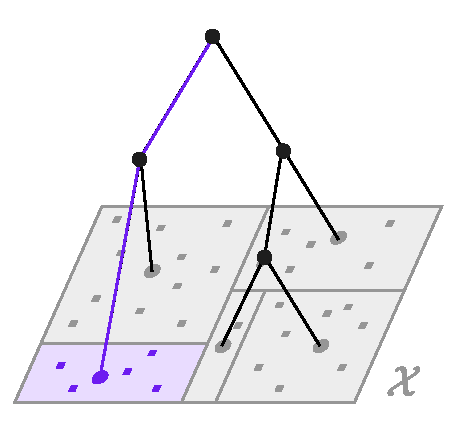
\includegraphics[width=\textwidth]{figma-illustrations/tree-partition.pdf}
    \label{fig:tree-partition}
    \caption{A decision tree partitioning the data space. For a query example, the corresponding leaf node is determined by traversing the tree downwards from the root node and applying the learned decision criteria.}
% TODO I think this fig does not really provide any value here
\end{marginfigure}

Decision Trees, particularly if grown deeply, can be considered to \textit{approximate} the training data, i.e. they are a lossy representation of the training data. A grown decision tree model contains two kinds of parameters, both derived from the training data $D$.
\begin{itemize}
\item The tree structure, i.e. the decision boundaries. These are used for determining the leaf node for a query example.
\item The output value of a leaf node. This is the predicted value for a query example falling into that leaf. The leaf predictions depend on the decision boundaries but are not solely determined by them. 
\end{itemize}
% TODO plot of approximated polynomial
This leads to the question whether characteristics of a Random Forest model could be expressed solely in terms of its tree parameters, and not in terms of predictions on query points.
% In the case of a forest of trees, one would expect that if the trees have different decision boundaries, the forest is more diverse. 
% Further, this would provide a way to express diversity \textit{in terms of model parameters} and not in terms of predictions on query points.
% In the case of a forest of trees, one would expect that if the trees have different decision boundaries, the forest is more diverse. 

\begin{marginfigure}
    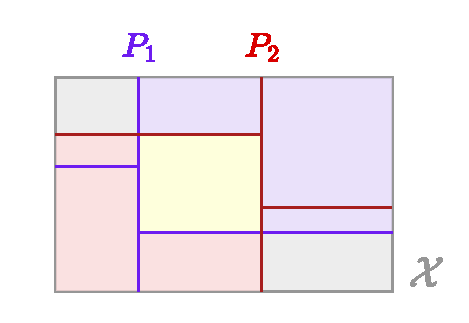
\includegraphics[width=\textwidth]{figma-illustrations/forest-partition.pdf}
    \label{fig:forest-partition}
    \caption{The data space $\mathcal{X}$ (gray) and partitions $P_1$ (purple) and $P_2$ (red) of it induced by two decision trees. The intersections of any cell of $P_1$ and any cell of $P_2$ form the \textit{forest partition}. One such intersection is highlighted in yellow.
    }
\end{marginfigure}
Each level of a decision tree induces a partition of the space of examples $\mathcal{X}$. Because each example is associated with an outcome, we can also think of it as a partition of $(\mathcal{X}, \mathcal{Y})$. We call such a partition a \textit{tree partition} and a cell a \textit{tree cell}.
Decision trees produce predictions via an aggregate of the queried leaf node's outcomes. Thus, the predictions of a decision tree over a single cell are constant.
An ensemble of trees also induces a partition: the partition obtained by intersecting all tree partitions. We call these \textit{forest cells}. Formally, if $T_{1}, \dots, T_{M}$ are tree partitions, the forest partition is given as
$$
\{ c_{1} \cap \dots \cap c_{M} ~|~ c_{1} \in T_{1}, \dots, c_{M} \in T_{M}\}
$$
Each forest cell is associated with $M$ tree cells whose intersection constitutes it.
For any query point that falls within a certain tree cell, the forest prediction is given by an aggregate over the associated tree cells. Thus, the predictions of a random forest are constant over a single forest cell.
This means that also a loss, as well as any decomposition constituents of the loss are constant over forest cells.

However, exploiting that partitions are cell-wise constant, we can apply a special case of the law of total expectation to express it in terms of cells.
\sidenote{
% TODO move to lemma in prelims
Let $X_{1} \dot\cup \dots \dot\cup X_{M}$ be a disjoint, countable partition of the sample space of $X$. Then
$$
\mathbb{E}_{X}\left[ X \right] = \sum_{i=1}^M  \mathbb{E}_{X}\left[ X ~|~X_{i} \right] \cdot \prob{}{X_{i}}
$$
}
Consider a forest partition $Z = Z_{1} \dot\cup \dots \dot\cup Z_{P}$ of $Z=(X,Y)$. Using the linearity of expectations and the law of total expectation, we can write the generalisation error of the forest as follows. 
$$
\mathbb{E}_{Z,D}\left[ \ell(y,\bar{q}) \right] = \mathbb{E}_{D}\left[ \sum_{p=1}^P \prob{}{Z_{p}} \cdot \mathbb{E}_{Z}\left[ \ell(y, \bar{q}) ~|~Z_{p}\right]   \right] 
$$
While we have eliminated the dependence on a query point $X$, the quantity $\mathbb{E}_{Z}\left[ \ell(y, \bar{q}) ~|~Z_{p}\right]$ still depends on a realisation of an outcome $Y$. In section \ref{sec:later} we will see that we can decompose this term further into components that are dependent and independent of $Y$, respectively.

\subsection{Practical advantages}
parallelisable, oob estimation, feature importance, proximity, ...

\end{document}